\documentclass[crop,tikz,convert={outext=.svg,command=\unexpanded{pdf2svg \infile\space\outfile}},multi=false]{standalone}[2012/04/13]

\usepackage[utf8]{inputenc}
\usepackage{amsmath, amssymb}
\usepackage{pgfplots}


%-------------------------------------
% Tikz and pgf options & definitions
%-------------------------------------
\pgfplotsset{compat=1.15}
\pgfmathsetseed{1}

\usetikzlibrary{positioning}
\usetikzlibrary{shapes}
\usetikzlibrary{backgrounds, fit}
\usetikzlibrary{calc}
\usetikzlibrary{decorations.markings}
\usetikzlibrary{matrix}

\def\colorvector at (#1,#2,#3){
\coordinate (A) at (#1, #2);
\filldraw[draw=black,fill=test!!+] (A)++(0,0) rectangle ++(0.25,0.25) node (A0) {};
\filldraw[draw=black,fill=test!!+] (A)++(0.3,0) rectangle ++(0.25,0.25) node (A1) {};
\filldraw[draw=black,fill=test!!+] (A)++(0.6,0) rectangle ++(0.25,0.25) node (A2) {};
\node[right=of A2, xshift=-7.5ex, yshift=-0.75ex] {$\ldots$};
\filldraw[draw=black,fill=test!!+] (A)++(1.5,0) rectangle ++(0.25,0.25) node (A4) {};
\node[left=of A1, xshift=4.4ex, yshift=-0.75ex] (BEG\i) {$#3=[$};
\node[right=of A4, xshift=-8ex, yshift=-0.75ex] (END\i) {$]^{T}$};
}

\begin{document}
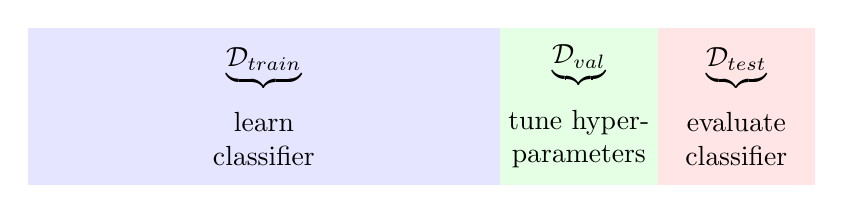
\begin{tikzpicture}
\path [fill=blue!10] (0,0) rectangle node[align=center, text width=2cm] {$\,\,\,\, \underbrace{{\cal D}_{train}}_{} \,\,\,\,$ learn classifier}(6,2) ;
\path [fill=green!10] (6,0) rectangle node[align=center, text width=2cm] {$\,\,\,\, \underbrace{{\cal D}_{val}}_{} \,\,\,\,$ tune hyper-parameters} (8,2);
\path [fill=red!10] (8,0) rectangle node[align=center, text width=2cm] {$\,\,\,\, \underbrace{{\cal D}_{test}}_{} \,\,\,\,$ evaluate classifier} (10,2);
\end{tikzpicture}
\end{document}